\chapter{Introduction}

In this report, we explore Hawkeye cache replacement and cache precleaning, two methods for improving performance of GPU memory systems. The first idea improves upon L1 and L2 cache replacement policies by implementing Hawkeye \cite{hawkeye}. Hawkeye learns from a delayed computation of the optimal cache replacement policy. The second idea, which we refer to as precleaning, avoids memory system stalls by commiting write-backs at a time of low bandwidth usage rather than at the time of eviction.

GPUs cater to highly parallel and regular data access patterns. While GPUs provide hardware specifically tailored for parallel problems, good GPU performance relies on programs exhibiting behavior that can be partitioned into thousands of highly regular threads executing the same code. Warps are what we call a collection of threads that run in lock-step, and all threads within a warp should run similar code and access relatively nearby data in memory. Data divergence occurs when these warps overload lower-level memory systems by exhibiting irregular access patterns and accessing multiple different cache lines simultaneously. Our goal in this paper, with both Hawkeye and precleaning, is to limit and offset the negative performance impacts of both data-divergence and poorly optimized data access patterns.

Computer architects have been using caches and smart cache replacement policies to hide the latency of predictable memory operations for decades \cite{deadblock,lruperf,cache_burst,dip,eva,rrip}. Caches ideally stores all data that will be accessed by the machine in the near future, hiding latency of memory accesses on the critical path. Unfortunately, cache memory is expensive and limited, thus architects rely on cache replacement policies to decide what data will be the most useful in the future.

Least Recently Used (LRU) is the baseline replacement policy for most caches as it is easy to reason about and performs well considering its relative simplicity. LRU does not store any information on lines previously evicted from the cache. Because of this lack of additional meta-data, LRU generally doesn't work well with access patterns with working sets that exceed the size of the cache. A cache with a more sophisticated replacement policy that can handle irregular or complex data access patterns can filter out some of the requests that would otherwise overload the GPU's main memory. By providing a proven approach to cache replacement on CPUs, we hope to improve performance on GPU programs that would previously see no benefit from the cache due to said programs’ data access patterns.

Our first idea for improving GPU memory system performance is to use Hawkeye, a CPU cache replacement policy that learns from the theoretically optimal cache replacement decisions for previous accesses to the cache. Hawkeye prefers to evict lines similar to other lower performing lines in the OPTGen algorithm, an online calculation of Belady’s optimal cache replacement policy. Hawkeye evaluates similarities between lines by comparing their defining features, such as warp ID and Program Counter (PC). Features help us correlate performance within OPTGen with future performance of lines with identical features. We also explore the application of Hawkeye in both the L1 and L2 caches.

Precleaning, our second idea for improving memory system performance, aims to spread out the bandwidth usage by writing back dirty cache lines at times of lower bandwidth usage. Write-through and write-back caches are the two main ways that modern caches handle mutable data within the cache. Write-through caches immediately write modified data back to their backing store (such as a lower level cache or DRAM). On the other hand, write-back caches delay committing writes to their backing store until the associated line is evicted. This delay in commiting writes is possible because non-atomic writes are off the critical path, meaning the processor will never need to stall for a non-atomic write. Write-back caches tend to be more efficient than write-through caches as write-through caches require an access to lower level memory for every single write. While the strategy of writing back at the last possible moment might be the most convenient, it is not necessarily the best time for data to be written back to lower level memory. Writing back at the time of eviction can be especially problematic in GPUs when unoptimized parallel code causes many simultaneous evictions. The key takeaway is that, rather than a binary choice of write-through and write-back, we actually have a full spectrum of choices to choose from when cleaning dirty cache lines. Please refer to Figure \ref{f:bandwidth_optimal} for a visualization of this spectrum.

\begin{figure}[htb]
\begin{center}
\ 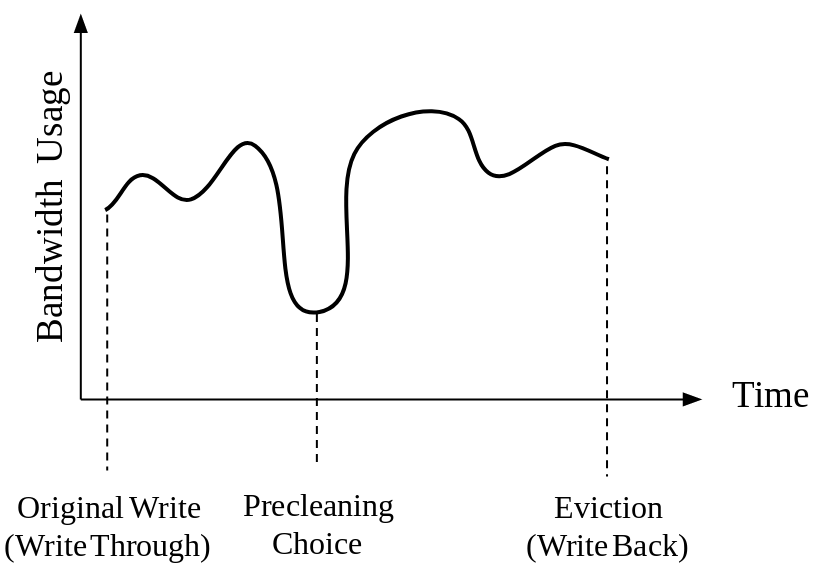
\psfig{file=figs/bandwidth_optimal.png,width=\textwidth}
\caption{Example of cache cleaning choices, showing potential improvement for bandwidth usage.}
\label{f:bandwidth_optimal}
\end{center}
\end{figure}
\index{commands!environments!figure}%

To further improve GPU memory system performance, we would like to use previous data and current memory bandwidth usage levels to determine a better time to write back modified cache lines. We believe that GPUs are a good fit for this problem due to the parallel nature of the hardware. Making accesses to memory across many cores increases the chances of multiple write-backs being triggered around the same time. GPUs rely on having adequate bandwidth available to hide latency across all cores. When bandwidth saturates, code executing on the GPU will effectively start to serialize, which negates the performance benefits of using a GPU. A perfect solution would evenly spread out all write-back traffic, preventing bandwidth spikes that could stall our GPU cores.
